\chapter{Background and related work}
\section{SDN and OpenFlow}
\label{SDN and OpenFlow}
OpenFlow is the most popular southbound interface in SDN. A switch that supports OpenFlow is called an OpenFlow switch. Aside from physical switches, there are also software implementations of virtual switches, such as \textit{Open vSwtich} (\url{openvswitch.org}). OpenFlow switches typically separate OpenFlow and non-OpenFlow traffic, which do not interfere with each other \cite{HP_SPEC}.

A controller is able to determine the forwarding path of packets by adding, updating and deleting flow entries in the flow tables of OpenFlow switches in both reactive and proactive ways \cite{OF_SPEC}. It also maintains the abstract view of the network, including network topology, host positions and the states of network resources. An incoming packet from the \textit{ingress port} will go through one or more flow tables, optionally through the group table, and be processed according to the actions defined by the matched flow entry. Each OpenFlow table typically contains hundreds of flow entries. Figure~\ref{FE_Col} presents the fields of a flow entry. Packets will be matched with the \textit{match fields} of a flow entry in the priority order. When a packet matches a flow entry, the action set to that packet will be modified according to the instructions in the entry, and the counter will record the match incident by increasing 1. After the end of the processing pipeline, the actions in the action set will be executed. We can also set timeout for an entry with the timeout field. The cookie is used as an identifier for flow entry. There is a new feature introduced in OpenFlow 1.5 -- the egress processing. Besides the original pipeline processing, the processing involves egress tables, which allows further matching and processing after executing the output action\cite{OF_SPEC}. 

\begin{figure}[H]
\begin{center} 
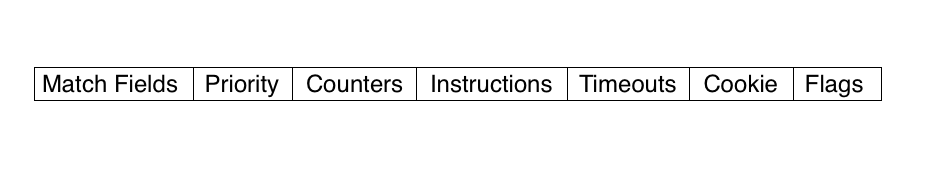
\includegraphics[width=1\textwidth]{figures/columns_of_flow_entry.png}
\end{center}
\caption{Fields of a flow entry.}
\label{FE_Col}
\end{figure}

Match fields of a flow entry have some complicated traits. A flow entry may have multiple match fields, e.g., \texttt{eth\_src} = \texttt{00:11:22:33:44:55}, \texttt{ipv4\_src} = \texttt{140.123.103.123}, \texttt{ipv4\_dst} = \texttt{140.123.103.124}, which mean a packet should contain all the above field values to be matched by the entry. When the action in a flow entry sends the packet to next table for further processing, the packet is also matched against more than one match field indirectly. Another advanced feature is the conjunction action that ties groups of individual flows with the same match field and different values into ``conjunctive flows'' to reduce the number of flow entries \cite{OVS_OFCTL}. There are also dependency requirements for match fields in OpenFlow. For example, it is not allowed to install a flow entry that has \texttt{ipv4\_src} as a match field without \texttt{eth\_type} equals to \texttt{0x0800}. The dependency requirements for some common match fields are shown in Table~\ref{table:match_fields_dependency}.

\begin{table}[H]
\centering
\caption{Common match fields and their dependency requirements}
\begin{tabular}{|l|l|l}
\hline Match field & Required dependent field(s) \\
\hline eth\_dst & None \\
\hline eth\_src & None \\
\hline ipv4\_src & eth\_type=0x0800 \\
\hline ipv4\_dst & eth\_type=0x0800 \\
\hline ipv6\_src & eth\_type=0x86DD \\
\hline ipv6\_dst & eth\_type=0x86DD \\
\hline tcp\_src & eth\_type=0x0800 or 0x86DD, ip\_proto=0x6 \\
\hline tcp\_dst & eth\_type=0x0800 or 0x86DD, ip\_proto=0x6 \\
\hline udp\_src & eth\_type=0x0800 or 0x86DD, ip\_proto=0x11 \\
\hline udp\_dst & eth\_type=0x0800 or 0x86DD, ip\_proto=0x11 \\
\hline icmpv4\_type & eth\_type=0x0800, ip\_proto=0x1 \\
\hline icmpv4\_code & eth\_type=0x0800, ip\_proto=0x1 \\
\hline icmpv6\_type & eth\_type=0x86DD, ip\_proto=0x3a \\
\hline icmpv6\_code & eth\_type=0x86DD, ip\_proto=0x3a \\
\hline
\end{tabular}
\label{table:match_fields_dependency}
\end{table}

There is usually a table-miss entry, which has the lowest priority and wildcards in all the match fields. It is for packets that cannot match any other flow entries. It does not exist by default, just like all other entries. The controller is able to add or remove it at any time. A packet will be dropped if it does not match any entry without a table-miss entry \cite{OF_SPEC}. Normally, such a packet will be encapsulated and sent to the controller using the controller-reserved port, and the controller will decide how to process it and add a new flow entry according to the network policy. 

\section{SDN security}
\label{SDN security}
A thorough review of SDN-related security issues can be found in \cite{LAB14, CM, SOS13, KJK}. Therefore, rather than repeat the review, we will focus on the issue of compromising OpenFlow switches, since it has been less addressed than the others so far. Compromising OpenFlow switches can lead to some negative results: (1) Attackers may launch topology poisoning attack by manipulating link discovery packets. (2) The actions of the flow entries on a compromised switch can be unexpectedly altered. (3) The packets that pass through a compromised switch can be eavesdropped or dropped. (4) The compromised switch may be configured to be managed by another malicious controller. (5) It is possible to launch network-wide denial-of-service attack by sending specific forged packets to consume the controller's resource.

\subsection{Topology poisoning attack}
The main idea of the topology poisoning attack is to trick the controller into believing the existence of a non-existing link to host or switch by exploiting traits of topology management service. One can initiate such type of attack with either a switch or a host. In \cite{HXWG15}, Hong et al. mentioned Host Location Hijacking Attack and Link Fabrication Attack, and presented TopoGuard to solve the problem. However, LLDP packets are passed around with the aid of switches. The Link Fabrication Attack can be also initiated by compromised switches, but the attack vector  is not covered in the scenario of TopoGuard. Bui gives three different attack scenarios of Link Fabrication Attack with compromised switches and evaluates their consequence under different routing algorithms and network topologies \cite{TTB15}. This attack is caused by the lack of authentication of LLDP. However, simply adding authenticator inside the LLDP packets will not help against LLDP relay attack \cite{HXWG15}. Alharbi et al. implement HMAC based mechanism with a little modification to static secret key, which is able to detect the injection of any fabricated LLDP packets, with only an acceptable of amount of overhead added \cite{ATPP15}.

\subsection{Unwanted flow entry modification}
Attackers can also modify the flow entries inside the flow tables of the compromised switch to perform MITM, eavesdropping or DOS attack \cite{AAS14}. The detection method proposed in \cite{CKGL15} is able to detect whether a switch is forwarding the packets in an unexpected way. After selecting a flow entry as the detecting target, they install new entries on its neighbors. With the match field selected by their algorithm, they are able to let every packet that matches the new flow entry matches the target flow entry. A packet containing the match field of the new flow entry will be sent from \texttt{Packet\_Out} to a neighbor of the target switch, forwarded to the target switch, go through the series of switches, and should be sent back to the controller. Finally, they will check if the packet comes back to the controller as expected and remains unchanged. However, this method will take a long time to run if it is desired to scan through a large number of flow entries. A pre-detection method to narrow down the potential targets is needed.

In \cite{PJL16}, Pang et al. discuss about forwarding anomaly and design a method to detect the problem. First, they find a minimal set of flows whose rule paths cover all flows. Next, additional dedicated flow entries with timeout will be installed, the actions of these dedicated entries will modify the label, and a label will be added into packets in order to collect flow statistics. The more dedicated entries are used, the more likely they are able to identify where the malicious flow entry is located. However, if the dedicated rules are installed right on the malicious switch, the newly-installed entry may be match in prior to the malicious entry and the method will not work. Therefore, they need to calculate the optimal number of dedicate entries to install in order to reach a balance between efficiency and probability to detect the malicious flow entries successfully. Their experimental result shows that FADE is able to detect forwarding anomaly in a network topology containing around 30 switches in 15 minutes with 2.5\% false negative and 4\% throughput reduction.

\subsection{Network debugging in SDN}
Although the main purpose is not identical, some network debugging methods can be quite inspiring for the development of malicious behavior detection method. Flow entry information gathering techniques can also be found in \cite{ARDC14}. Just like traceroute, Agarwal et al. aim to trace the traveling path of a packet in a SDN network with minimal influence to the network. They use vlan field as color labels of switches. By setting up entries with color as match field in the way specified in \cite{ARDC14}, they are able to match the incoming probing packets from other switches and send them to the controller for logging, while not matching the probing packets from the controller and use the actual forwarding rules in the switch. Normally, the probing procedure repeats until the packet is consumed by a host or meets a loop. However, when malicious behaviors like packet dropping occur, it is also likely to find the culprit by checking the last hop of the probing packet.

Automatic Test Packet Generation (ATPG) proposed in \cite{ZKVM12} is able to test through tremendous number of flow rules and links with the packets less than 1\% of the traffic in an automatic way. They use ``rules'' to define how packets should be processed, and keep a list of rule histories for each pair of ingress and egress port. Similar to \cite{PJL16}, they find the minimal subset of test packets whose travel path covers the detection objective (entries, links or router queues), and check the packets to see if the actions are executed normally when it reach an end point. Since that work runs on regular networks, it requires deployment of terminals for generating test packets. In contrast, we utilize the trait of action set in OpenFlow and deploy new flow entries that are able to duplicate detection packets from a switch and send them to other switches in a tree-like manner. This increases the number of entries a single detection packet is able to detect. 

\subsection{Other attacks}
By intercepting the control channel without complete TLS with a compromised switch, an attacker is able to spoof messages and effect whole network. For example, one may also reconfigure a compromised switch to use an attacker-controlled controller than the one it should. This type of attack is called Control-channel hijacking attack.

An attacker can tell if a new flow entry is installed by sending packets and observing the response time. \cite{BCKK15}. With this method, one can fingerprint the flow entries inside the OpenFlow switches and perform a DOS to the controller by deliberately crafting malicious packets for controller to process slowly with a switch or host\cite{AAS14}.
